\documentclass[12pt]{report}
\usepackage{suthesis}
%\documentstyle[12pt,suthesis]{report}

% -- Imports --
% (general libraries)
\usepackage{times,latexsym,amsfonts,amssymb,amsmath,graphicx,url,bbm,rotating}
\usepackage{multirow,hhline,stmaryrd,bussproofs,mathtools,siunitx}
\usepackage{booktabs,xcolor,csquotes,calligra}
\usepackage{mhchem}
% (custom libraries)
\usepackage{afterpage}
\usepackage{longtable}
\usepackage{fitch}
% (inline references)
\usepackage{natbib}
\usepackage{tabularx}
\usepackage[hidelinks]{hyperref}
\hypersetup{
    colorlinks=true,
    citecolor=magenta,
    linkcolor=.,
    urlcolor=blue
}

\usepackage{epigraph}
\renewcommand{\epigraphsize}{\normalsize}
\setlength{\epigraphwidth}{0.9\textwidth}

% (tikz)
\usepackage{soul}
\definecolor{light-yellow}{RGB}{255, 255, 153}
\sethlcolor{light-yellow}
\usepackage{tikz}
\usepackage{tikz-dependency,pifont}
\usetikzlibrary{shapes.arrows,chains,positioning,automata,trees,calc}
\usetikzlibrary{patterns,matrix}
\usetikzlibrary{decorations.pathmorphing,decorations.markings}
% (print algorithms)
\usepackage[ruled,lined,linesnumbered]{algorithm2e}
% (custom)
% version 1.2 05/21/08
\newcommand\sa{\ensuremath{\mathcal{a}}}
\newcommand\sd{\ensuremath{\mathcal{d}}}
\newcommand\se{\ensuremath{\mathcal{e}}}
\newcommand\sg{\ensuremath{\mathcal{g}}}
\newcommand\sh{\ensuremath{\mathcal{h}}}
\newcommand\seye{\ensuremath{\mathcal{i}}}
\newcommand\sj{\ensuremath{\mathcal{j}}}
\newcommand\sk{\ensuremath{\mathcal{k}}}
\newcommand\sm{\ensuremath{\mathcal{m}}}
\newcommand\sn{\ensuremath{\mathcal{n}}}
\newcommand\sq{\ensuremath{\mathcal{q}}}
\newcommand\sr{\ensuremath{\mathcal{r}}}
\newcommand\su{\ensuremath{\mathcal{u}}}
\newcommand\sv{\ensuremath{\mathcal{v}}}
\newcommand\sw{\ensuremath{\mathcal{w}}}
\newcommand\sx{\ensuremath{\mathcal{x}}}
\newcommand\sy{\ensuremath{\mathcal{y}}}
\newcommand\sz{\ensuremath{\mathcal{z}}}
\newcommand\sA{\ensuremath{\mathcal{A}}}
\newcommand\sB{\ensuremath{\mathcal{B}}}
\newcommand\sC{\ensuremath{\mathcal{C}}}
\newcommand\sD{\ensuremath{\mathcal{D}}}
\newcommand\sE{\ensuremath{\mathcal{E}}}
\newcommand\sF{\ensuremath{\mathcal{F}}}
\newcommand\sG{\ensuremath{\mathcal{G}}}
\newcommand\sH{\ensuremath{\mathcal{H}}}
\newcommand\sI{\ensuremath{\mathcal{I}}}
\newcommand\sJ{\ensuremath{\mathcal{J}}}
\newcommand\sK{\ensuremath{\mathcal{K}}}
\newcommand\sL{\ensuremath{\mathcal{L}}}
\newcommand\sM{\ensuremath{\mathcal{M}}}
\newcommand\sN{\ensuremath{\mathcal{N}}}
\newcommand\sO{\ensuremath{\mathcal{O}}}
\newcommand\sP{\ensuremath{\mathcal{P}}}
\newcommand\sQ{\ensuremath{\mathcal{Q}}}
\newcommand\sR{\ensuremath{\mathcal{R}}}
\newcommand\sS{\ensuremath{\mathcal{S}}}
\newcommand\sT{\ensuremath{\mathcal{T}}}
\newcommand\sU{\ensuremath{\mathcal{U}}}
\newcommand\sV{\ensuremath{\mathcal{V}}}
\newcommand\sW{\ensuremath{\mathcal{W}}}
\newcommand\sX{\ensuremath{\mathcal{X}}}
\newcommand\sY{\ensuremath{\mathcal{Y}}}
\newcommand\sZ{\ensuremath{\mathcal{Z}}}
\newcommand\ba{\ensuremath{\mathbf{a}}}
\newcommand\bb{\ensuremath{\mathbf{b}}}
\newcommand\bc{\ensuremath{\mathbf{c}}}
\newcommand\bd{\ensuremath{\mathbf{d}}}
\newcommand\be{\ensuremath{\mathbf{e}}}
\newcommand\bef{\ensuremath{\mathbf{f}}}
\newcommand\bg{\ensuremath{\mathbf{g}}}
\newcommand\bh{\ensuremath{\mathbf{h}}}
\newcommand\bi{\ensuremath{\mathbf{i}}}
\newcommand\bj{\ensuremath{\mathbf{j}}}
\newcommand\bk{\ensuremath{\mathbf{k}}}
\newcommand\bl{\ensuremath{\mathbf{l}}}
\newcommand\bn{\ensuremath{\mathbf{n}}}
\newcommand\bo{\ensuremath{\mathbf{o}}}
\newcommand\bp{\ensuremath{\mathbf{p}}}
\newcommand\bq{\ensuremath{\mathbf{q}}}
\newcommand\br{\ensuremath{\mathbf{r}}}
\newcommand\bs{\ensuremath{\mathbf{s}}}
\newcommand\bt{\ensuremath{\mathbf{t}}}
\newcommand\bu{\ensuremath{\mathbf{u}}}
\newcommand\bv{\ensuremath{\mathbf{v}}}
\newcommand\bw{\ensuremath{\mathbf{w}}}
\newcommand\bx{\ensuremath{\mathbf{x}}}
\newcommand\by{\ensuremath{\mathbf{y}}}
\newcommand\bz{\ensuremath{\mathbf{z}}}
\newcommand\bA{\ensuremath{\mathbf{A}}}
\newcommand\bB{\ensuremath{\mathbf{B}}}
\newcommand\bC{\ensuremath{\mathbf{C}}}
\newcommand\bD{\ensuremath{\mathbf{D}}}
\newcommand\bE{\ensuremath{\mathbf{E}}}
\newcommand\bF{\ensuremath{\mathbf{F}}}
\newcommand\bG{\ensuremath{\mathbf{G}}}
\newcommand\bH{\ensuremath{\mathbf{H}}}
\newcommand\bI{\ensuremath{\mathbf{I}}}
\newcommand\bJ{\ensuremath{\mathbf{J}}}
\newcommand\bK{\ensuremath{\mathbf{K}}}
\newcommand\bL{\ensuremath{\mathbf{L}}}
\newcommand\bM{\ensuremath{\mathbf{M}}}
\newcommand\bN{\ensuremath{\mathbf{N}}}
\newcommand\bO{\ensuremath{\mathbf{O}}}
\newcommand\bP{\ensuremath{\mathbf{P}}}
\newcommand\bQ{\ensuremath{\mathbf{Q}}}
\newcommand\bR{\ensuremath{\mathbf{R}}}
\newcommand\bS{\ensuremath{\mathbf{S}}}
\newcommand\bT{\ensuremath{\mathbf{T}}}
\newcommand\bU{\ensuremath{\mathbf{U}}}
\newcommand\bV{\ensuremath{\mathbf{V}}}
\newcommand\bW{\ensuremath{\mathbf{W}}}
\newcommand\bX{\ensuremath{\mathbf{X}}}
\newcommand\bY{\ensuremath{\mathbf{Y}}}
\newcommand\bZ{\ensuremath{\mathbf{Z}}}
\newcommand\Ba{\ensuremath{\mathbb{a}}}
\newcommand\Bb{\ensuremath{\mathbb{b}}}
\newcommand\Bc{\ensuremath{\mathbb{c}}}
\newcommand\Bd{\ensuremath{\mathbb{d}}}
\newcommand\Be{\ensuremath{\mathbb{e}}}
\newcommand\Bf{\ensuremath{\mathbb{f}}}
\newcommand\Bg{\ensuremath{\mathbb{g}}}
\newcommand\Bh{\ensuremath{\mathbb{h}}}
\newcommand\Bi{\ensuremath{\mathbb{i}}}
\newcommand\Bj{\ensuremath{\mathbb{j}}}
\newcommand\Bk{\ensuremath{\mathbb{k}}}
\newcommand\Bl{\ensuremath{\mathbb{l}}}
\newcommand\Bm{\ensuremath{\mathbb{m}}}
\newcommand\Bn{\ensuremath{\mathbb{n}}}
\newcommand\Bo{\ensuremath{\mathbb{o}}}
\newcommand\Bp{\ensuremath{\mathbb{p}}}
\newcommand\Bq{\ensuremath{\mathbb{q}}}
\newcommand\Br{\ensuremath{\mathbb{r}}}
\newcommand\Bs{\ensuremath{\mathbb{s}}}
\newcommand\Bt{\ensuremath{\mathbb{t}}}
\newcommand\Bu{\ensuremath{\mathbb{u}}}
\newcommand\Bv{\ensuremath{\mathbb{v}}}
\newcommand\Bw{\ensuremath{\mathbb{w}}}
\newcommand\Bx{\ensuremath{\mathbb{x}}}
\newcommand\By{\ensuremath{\mathbb{y}}}
\newcommand\Bz{\ensuremath{\mathbb{z}}}
\newcommand\BA{\ensuremath{\mathbb{A}}}
\newcommand\BB{\ensuremath{\mathbb{B}}}
\newcommand\BC{\ensuremath{\mathbb{C}}}
\newcommand\BD{\ensuremath{\mathbb{D}}}
\newcommand\BE{\ensuremath{\mathbb{E}}}
\newcommand\BF{\ensuremath{\mathbb{F}}}
\newcommand\BG{\ensuremath{\mathbb{G}}}
\newcommand\BH{\ensuremath{\mathbb{H}}}
\newcommand\BI{\ensuremath{\mathbb{I}}}
\newcommand\BJ{\ensuremath{\mathbb{J}}}
\newcommand\BK{\ensuremath{\mathbb{K}}}
\newcommand\BL{\ensuremath{\mathbb{L}}}
\newcommand\BM{\ensuremath{\mathbb{M}}}
\newcommand\BN{\ensuremath{\mathbb{N}}}
\newcommand\BO{\ensuremath{\mathbb{O}}}
\newcommand\BP{\ensuremath{\mathbb{P}}}
\newcommand\BQ{\ensuremath{\mathbb{Q}}}
\newcommand\BR{\ensuremath{\mathbb{R}}}
\newcommand\BS{\ensuremath{\mathbb{S}}}
\newcommand\BT{\ensuremath{\mathbb{T}}}
\newcommand\BU{\ensuremath{\mathbb{U}}}
\newcommand\BV{\ensuremath{\mathbb{V}}}
\newcommand\BW{\ensuremath{\mathbb{W}}}
\newcommand\BX{\ensuremath{\mathbb{X}}}
\newcommand\BY{\ensuremath{\mathbb{Y}}}
\newcommand\BZ{\ensuremath{\mathbb{Z}}}
\newcommand\balpha{\ensuremath{\mbox{\boldmath$\alpha$}}}
\newcommand\bbeta{\ensuremath{\mbox{\boldmath$\beta$}}}
\newcommand\btheta{\ensuremath{\mbox{\boldmath$\theta$}}}
\newcommand\bphi{\ensuremath{\mbox{\boldmath$\phi$}}}
\newcommand\bpi{\ensuremath{\mbox{\boldmath$\pi$}}}
\newcommand\bpsi{\ensuremath{\mbox{\boldmath$\psi$}}}
\newcommand\bmu{\ensuremath{\mbox{\boldmath$\mu$}}}
% Basic
\newcommand\T{\text}
\newcommand\sign{\text{sign}}
\newcommand\tr{\text{tr}}
\newcommand\fig[1]{\begin{center} \includegraphics{#1} \end{center}}
\newcommand\Fig[5]{\begin{figure}[tb] \begin{center} \includegraphics[scale=#2]{#1} \end{center} \longcaption{#4}{\label{fig:#3} #5} \end{figure}}
\newcommand\FigTop[4]{\begin{figure}[t] \begin{center} \includegraphics[scale=#2]{#1} \end{center} \caption{\label{fig:#3} #4} \end{figure}}
\newcommand\FigStar[4]{\begin{figure*}[tb] \begin{center} \includegraphics[scale=#2]{#1} \end{center} \caption{\label{fig:#3} #4} \end{figure*}}
\newcommand\aside[1]{\quad\text{[#1]}}
\newcommand\homework[3]{\title{#1} \author{#2} \date{#3} \maketitle}
% Math
\newcommand\argmin{\mathop{\text{argmin}}}
\newcommand\argmax{\mathop{\text{argmax}}}
\newcommand\p[1]{\ensuremath{\left( #1 \right)}} % Parenthesis ()
\newcommand\pb[1]{\ensuremath{\left[ #1 \right]}} % []
\newcommand\pc[1]{\ensuremath{\left\{ #1 \right\}}} % {}
\newcommand\eval[2]{\ensuremath{\left. #1 \right|_{#2}}} % Evaluation
\newcommand\inv[1]{\ensuremath{\frac{1}{#1}}}
\newcommand\half{\ensuremath{\frac{1}{2}}}
\newcommand\R{\ensuremath{\mathbb{R}}} % Real numbers
\newcommand\Z{\ensuremath{\mathbb{Z}}} % Integers
\newcommand\inner[2]{\ensuremath{\left< #1, #2 \right>}} % Inner product
\newcommand\mat[2]{\ensuremath{\left(\begin{array}{#1}#2\end{array}\right)}} % Matrix
\newcommand\eqn[1]{\begin{eqnarray} #1 \end{eqnarray}} % Equation (array)
\newcommand\eqnl[2]{\begin{eqnarray} \label{eqn:#1} #2 \end{eqnarray}} % Equation (array) with label
\newcommand\eqdef{\ensuremath{\stackrel{\rm def}{=}}} % Equal by definition
%\newcommand{\1}{\mathbb{I}} % Indicator (don't use \mathbbm{1} because bbm is not TrueType though)
\newcommand{\1}{\ensuremath{\mathbbm{1}}}
\newcommand{\bone}{\mathbf{1}} % for vector one
\newcommand{\bzero}{\mathbf{0}} % for vector zero
\newcommand\refeqn[1]{(\ref{eqn:#1})}
\newcommand\refeqns[2]{(\ref{eqn:#1}) and (\ref{eqn:#2})}
\newcommand\refchp[1]{Chapter~\ref{chp:#1}}
\newcommand\refsec[1]{Section~\ref{sec:#1}}
\newcommand\refsecs[2]{Sections~\ref{sec:#1} and~\ref{sec:#2}}
\newcommand\reffig[1]{Figure~\ref{fig:#1}}
\newcommand\reffigs[2]{Figures~\ref{fig:#1} and~\ref{fig:#2}}
\newcommand\reffigss[3]{Figures~\ref{fig:#1},~\ref{fig:#2}, and~\ref{fig:#3}}
\newcommand\reffigsss[4]{Figures~\ref{fig:#1},~\ref{fig:#2},~\ref{fig:#3}, and~\ref{fig:#4}}
\newcommand\reftab[1]{Table~\ref{tab:#1}}
\newcommand\refapp[1]{Appendix~\ref{sec:#1}}
\newcommand\refthm[1]{Theorem~\ref{thm:#1}}
\newcommand\refthms[2]{Theorems~\ref{thm:#1} and~\ref{thm:#2}}
\newcommand\reflem[1]{Lemma~\ref{lem:#1}}
\newcommand\reflems[2]{Lemmas~\ref{lem:#1} and~\ref{lem:#2}}
\newcommand\refprop[1]{Proposition~\ref{prop:#1}}
\newcommand\refdef[1]{Definition~\ref{def:#1}}
\newcommand\refcor[1]{Corollary~\ref{cor:#1}}
\newcommand\refalg[1]{Algorithm~\ref{alg:#1}}

\newcommand\Chapter[2]{\chapter{#2}\label{chp:#1}}
\newcommand\Section[2]{\section{#2}\label{sec:#1}}
\newcommand\Subsection[2]{\subsection{#2}\label{sec:#1}}
\newcommand\Subsubsection[2]{\subsubsection{#2}\label{sec:#1}}
%\newtheorem{definition}{Definition}
%\newtheorem{assumption}{Assumption}
%\newtheorem{proposition}{Proposition}
%\newtheorem{theorem}{Theorem}
%\newtheorem{lemma}{Lemma}
%\newtheorem{corollary}{Corollary}
% Probability
\newcommand\cv{\ensuremath{\to}} % Convergence
\newcommand\cvL{\ensuremath{\xrightarrow{\mathcal{L}}}} % Convergence in law
\newcommand\cvd{\ensuremath{\xrightarrow{d}}} % Convergence in distribution
\newcommand\cvP{\ensuremath{\xrightarrow{P}}} % Convergence in probability
\newcommand\cvas{\ensuremath{\xrightarrow{a.s.}}} % Convergence almost surely
\newcommand\eqdistrib{\ensuremath{\stackrel{d}{=}}} % Equal in distribution
\newcommand\E[1]{\ensuremath{\mathbb{E}{\left[#1\right]}}} % Expectation
\newcommand\Ex[2]{\ensuremath{\mathbb{E}_{#1}\left[#2\right]}} % Expectation
%\newcommand\var{\ensuremath{\text{var}}} % Variance
\newcommand\cov{\ensuremath{\text{cov}}} % Covariance
\newcommand\diag{\ensuremath{\text{diag}}} % Diagnonal matrix
\newcommand\cE[2]{\ensuremath{\E \left( #1 \mid #2 \right)}} % Conditional expectation
\newcommand\KL[2]{\ensuremath{\T{KL}\left( #1 \,||\, #2 \right)}} % KL-divergence
\newcommand\D[2]{\ensuremath{\bD\left( #1 \,||\, #2 \right)}} % KL-divergence

% Utilities
\newcommand\lte{\leq}
\newcommand\gte{\geq}
\newcommand\lone[1]{\ensuremath{\|#1\|_1}}
\newcommand\ltwo[1]{\ensuremath{\|#1\|_2^2}}
\newcommand\naive{na\"{\i}ve}
\newcommand\Naive{Na\"{\i}ve}

% Debug
\usepackage{color}
\newcommand{\tred}[1]{\textcolor{red}{#1}}
\newcommand{\hly}[1]{\hl{yellow}{#1}}
% \def\todo#1{\hl{{\bf TODO:} #1}{yellow}}
\def\needcite{\hl{{$^{\tt\small[citation\ needed]}$}}{blue}}
\def\needfig{\hl{Figure X}{green}}
\def\needtab{\hl{Table Y}{green}}
\def\note#1{\hl{{\bf NOTE:} #1}{yellow}}
\def\dome{\hl{{\bf TODO:} write me!}{yellow}}

% (tweaks)
\definecolor{darkred}{rgb}{0.5451, 0.0, 0.0}
\definecolor{darkgreen}{rgb}{0.0, 0.3922, 0.0}

\def\blue#1{\textcolor{blue}{#1}}
\def\darkblue#1{\textcolor{blue}{#1}}
\def\red#1{\textcolor{red}{#1}}
\def\darkred#1{\textcolor{darkred}{#1}}
\def\green#1{\textcolor{green}{#1}}
\def\darkgreen#1{\textcolor{darkgreen}{#1}}
\def\yellow#1{\textcolor{yellow}{#1}}
\definecolor{burntorange}{HTML}{BF5700}
\def\orange#1{\textcolor{burntorange}{#1}}
\def\gray#1{\textcolor{gray}{#1}}
\def\darkgray#1{\textcolor{darkgray}{#1}}

\newcommand\sys[1]{\textsc{#1}}
\newcommand\ti[1]{\textit{#1}}
\newcommand\tf[1]{\textbf{#1}}
\newcommand\mf[1]{\mathbf{#1}}
\newcommand{\indentitem}{\setlength\itemindent{25pt}}
\newcommand{\nth}{$^{\textrm{th}}$}

\newcommand\denote[1]{\ensuremath{\llbracket\ti{#1}\rrbracket}}

\newcommand\forward{\ensuremath{\sqsubseteq}}
\newcommand\nforward{\ensuremath{\not\sqsubseteq}}
\newcommand\reverse{\ensuremath{\sqsupseteq}}
\newcommand\alternate{\ensuremath{\downharpoonleft\hspace{-1.25mm}\upharpoonright}}
\newcommand\cover{\ensuremath{\smallsmile}}
\newcommand\equivalent{\ensuremath{\equiv}}
\newcommand\negate{\ensuremath{\curlywedge}}
\newcommand\independent{\ensuremath{\#}}
\newcommand\tagUp[1]{#1\ensuremath{^\uparrow}}
\newcommand\tagDown[1]{#1\ensuremath{^\downarrow}}
\newcommand\join{\ensuremath{\bowtie}}

\newcommand\h[1]{\textbf{#1}}
\newcommand\hh[1]{\textbf{\textcolor[rgb]{0.5,0,0}{#1}}}
\def\ent#1{\text{\small{\textsc{#1}}}}
\def\typ#1{\textit{#1}}
%\makeatletter
%\newcommand{\xRightarrow}[2][]{\ext@arrow 0359\Rightarrowfill@{#1}{#2}}
%\makeatother

\def\checkmark{\tikz\fill[scale=0.4](0,.35) -- (.25,0) -- (1,.7) -- (.25,.15) -- cycle;}
\newcommand{\xmark}{\textrm{\ding{55}}}
%\newcommand{\valid}{\ensuremath{\Rightarrow}}
%\newcommand{\invalid}{\ensuremath{\Rightarrow\lnot}}
\newcommand{\valid}{\ensuremath{\Leftarrow}}
\newcommand{\invalid}{\reflectbox{\ensuremath{\Rightarrow\lnot}}}
\newcommand{\noop}{\textcolor{white}{NOOP}}
\newcommand{\noopTab}{\begin{tabular}{c} \textcolor{white}{NOOP} \\ \textcolor{white}{NOOP} \end{tabular}}

\newcommand\true[1]{\darkgreen{\checkmark\textit{#1}}}
\newcommand\false[1]{\darkred{\xmark$~\,$\textit{#1}}}
\newcommand\unknown[1]{?\orange{\textit{#1}}}

\newcommand{\verticalcenter}[1]{\begingroup
\setbox0=\hbox{#1}%
\parbox{\wd0}{\box0}\endgroup}


%
% KBP MACROS
%
% A variable, abstracted (e.g., x)
\def\var#1{\ensuremath{\mathbf{{#1}}}}
% A variable instance (e.g., Obama)
\def\vari#1{\ensuremath{#1}}


% Aliases
\def\reverb{ReVerb}
\def\hydra{Stanford KBP}
\def\knowbot{\sys{Knowbot}}


% KBP Specific
% An entity
\def\ent#1{\text{\small{\textsc{#1}}}}

% An extraction, e.g., "Obama born_in Hawaii"
\newcommand\extr[3]{\mbox{\ent{#1}\ $~$\rel{#2}\ $~$\ent{#3}}}
\newcommand\triple[3]{(\mbox{\ent{#1}; $~$\rel{#2}; $~$\ent{#3}})}
% A clause in a logical form, e.g., "born_in(Obama, Hawaii)"
\newcommand\clause[3]{\mbox{\rel{#2}\ensuremath{(#1, #3)}}}

\newcommand\subj[1]{\textcolor{darkblue}{#1}}
\newcommand\obj[1]{\textcolor{burntorange}{#1}}
\newcommand\rel[1]{\textrm{#1}}

\def\blue#1{\textcolor{blue}{#1}}
\def\red#1{\textcolor{red}{#1}}
\def\green#1{\textcolor{green}{#1}}
\def\yellow#1{\textcolor{yellow}{#1}}

\newcommand\posterline{
  \begin{center}
    \noindent\rule{10cm}{0.4pt}
  \end{center}
}

\newcommand\entailmentExample[2]{
\vspace{0.5cm}
\noindent \hspace{0.5cm}\begin{tabular}{lp{0.80\textwidth}}
\textbf{P}: & \hspace*{-1mm}\textit{#1} \\
\textbf{H}: & \hspace*{-1mm}\textit{#2}
\end{tabular}
\vspace{0.5cm}
}

\tikzset{
    invisible/.style={opacity=0},
    visible on/.style={alt=#1{}{invisible}},
    alt/.code args={<#1>#2#3}{%
      \alt<#1>{\pgfkeysalso{#2}}{\pgfkeysalso{#3}} % \pgfkeysalso doesn't change the path
    },
  }

\newenvironment{lquote}{%
  \list{}{%
    \rightmargin0pt}%
    \item\relax
  }
{\endlist}

\newcommand\circled[1]{\tikz[baseline=(char.base)]{
            \node[shape=circle,draw=darkred,inner sep=2pt] (char) {#1};}
}
\newcommand\noncircled[1]{\tikz[baseline=(char.base)]{
            \node[shape=circle,draw=white,inner sep=2pt] (char) {#1};}
}


\newcommand{\hnode}[1]{|(#1)| \w{#1}}
\newcommand{\rnode}[2]{|(#1#2)| \w{\textcolor{darkblue}{\textbf{#1}}}\textcolor{white}{#2}}
\newcommand{\bnode}[2]{|(#1#2)| \w{\textcolor{darkblue}{\textcolor{darkred}{\textbf{#1}}}}\textcolor{white}{#2}}


\newcommand\longcaption[2]{\caption[#1]{#2}}


% (paper compilation hacks)
\def\newcite#1{\citet{#1}}
\def\cite#1{\citep{#1}}
%\def\newcite#1{\textcite{#1}}
%\def\cite#1{\autocite{#1}}
\definecolor{darkblue}{rgb}{0.0,0.0,0.4}


% Common hyphenations
\hyphenation{Text-Runner}
\hyphenation{Verb-Ocean}
\hyphenation{Raj-pur-kar}

%\bibliographystyle{plainnat}


% Comments
\usepackage{xspace}
\usepackage{xargs} % commandx
\usepackage[colorinlistoftodos,prependcaption,textsize=tiny]{todonotes}
\usepackage{marginnote}
\usepackage{color}
\definecolor{darkgreen}{RGB}{0,100,0}

% Inline comments useful for tables and figures.
\newcommandx{\icmtl}[2][1=]{\todo[inline]{DC: #2}\xspace}
\newcommandx{\icmtm}[2][1=]{\todo[inline]{CM: #2}\xspace}

% Comments for other places.
\newcommandx{\cmtl}[2][1=]{\todo[linecolor=blue,backgroundcolor=blue!10,bordercolor=blue,#1]{DC: #2}\xspace}
\newcommandx{\cmtm}[2][1=]{\todo[linecolor=red,backgroundcolor=red!10,bordercolor=red,#1]{CM: #2}\xspace}

\newcommand\cmb[1]{\marginpar{\tiny\raggedright\textcolor{blue}{\textsf{ DC\@: #1}}}}
\newcommand\cmm[1]{\marginpar{\tiny\raggedright\textcolor{red}{\textsf{\bfseries CM\@: #1}}}}

\usepackage{enumerate}

\setcounter{secnumdepth}{3}

\usepackage{footnote}
\makesavenoteenv{tabular}
\makesavenoteenv{table}

\usepackage{xpinyin}

% -- Document --
\begin{document}

% UCL Logo
\vspace*{-5cm}
\hspace*{-1.35cm}
\makebox[\textwidth]{
\includegraphics[width=\paperwidth]{img/_UCL_Banner-a4-port-black.eps}}
\vfill % Elastic empty space filler

% Title
\title{An Image Recognition Algorithm Approach to Distinguishing and Categorising the Small-Boat Fleet in the Gulf of California}
\author{UCL Candidate Code: KNCM2}
\principaladviser{Santiago Suarez De LaFuente}

% Preface
\beforepreface
%%!TEX root = thesis.tex

\prefacesection{Abstract}

Teaching machines to recognize and even understand satellite images is one of the most elusive and persistent challenges in artificial intelligence. This thesis tackles satellite image recognition: using the data and models needed to train models to identify small boats and measure their length. On the one hand, detecting small boats in satellite images is a major test of artificial intelligence algorithms. But, on the other hand, if we can build efficient object detection models, it will become a key technology for building carbon inventories in the shipping industry.

This thesis focuses on convolutional neural network models: a class of neural network models built on top of convolutional operations. These end-to-end neural models are more effective in learning media content (e.g., texts, images, and videos) and substantially improve performance on all object detection benchmarks than traditional feature-based models.

This thesis consists of two parts. In the first part, our goal is to cover every aspect of object detection algorithm and show our efforts in building effective object detection models and, more importantly, to understand what convolutional neural network models have actually learned. In the second part of this thesis, I show my detection results and analyze the various possibilities behind the results.

In particular, I discuss two new research directions at the end of this thesis: 1) whether a CAD model can replace the data from the training model, and 2) whether the algorithm has the ability (memory and understanding) to identify the same ship that appears at different times. I believe that they hold great promise for future satellite image analysis.
%%!TEX root = thesis.tex

\prefacesection{Acknowledgments}


\newpage

\begin{flushright}
%To my parents and Shiyi, for their unconditional love.
\end{flushright}

\afterpreface
\hypersetup{linkcolor=magenta}


% -- Sections --
% Introduction
\chapter{Introduction}
\label{chapter:intro}
%!TEX root = thesis.tex

\section{Motivation}
\subsection{Energy Crisis, Resources and Climate Change}
The energy crisis is one of the most essential and critical crises in the 21st century. Due to the growth of population and the increase of energy intensity per capita, a shortage of energy supply has occurred frequently in recent years, which often causes an energy crisis, usually involving scarcity of oil, electricity or other natural resources. Nowadays, non-renewable resource still consists of a large proportion in the energy system. According to BP Statistical Review of World Energy \& Ember (see Figure~\ref{intro_renewable}), the share of electricity production from renewables has continued growing since 2007. In 2020, the share of electricity production from renewables was around 29\% (see Figure~\ref{intro_renewable}). In other words, non-renewasbles are still the majority sources of electricity production today, although the share of them is shrinking.\\


\begin{figure}
\center
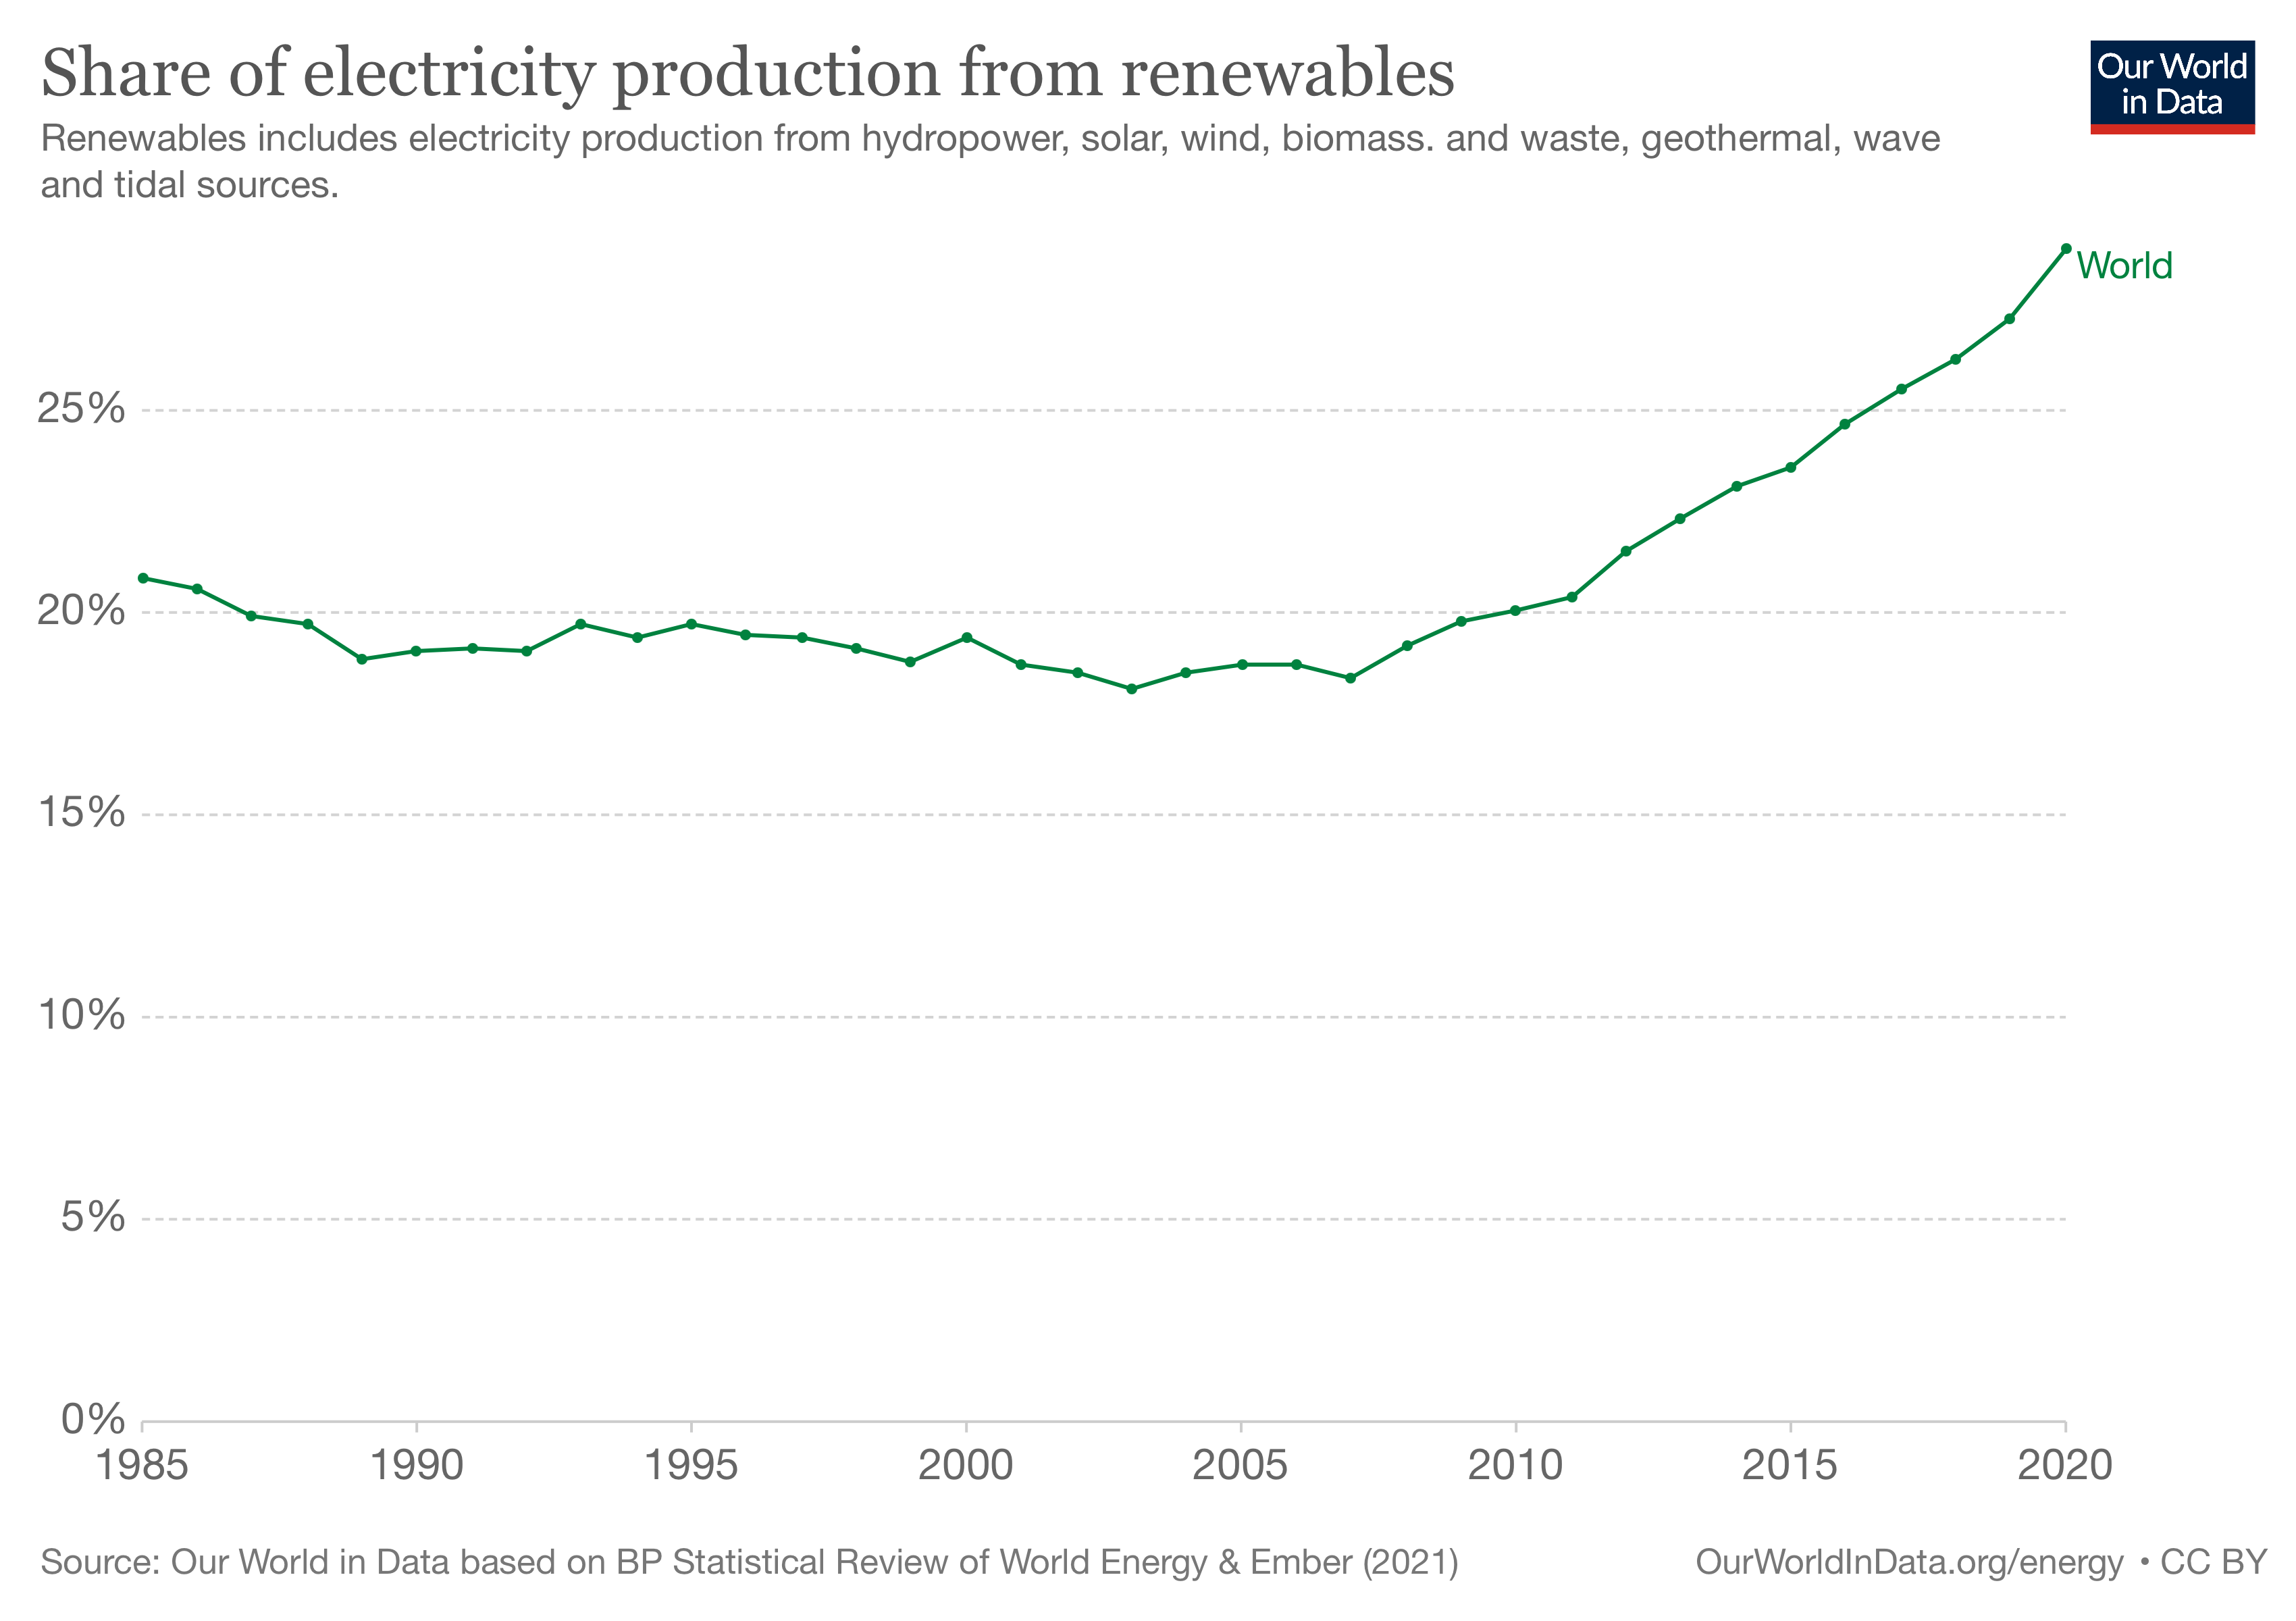
\includegraphics[scale=0.11]{img/intro_renewable.png}
\caption{The share of electricity production from renewables increased from around 18\% to 21\% during 1985 to 2007~\cite{BP2021bp}. The share of electricity production from renewables has been continued growing since 2007. In 2020, the share of electricity production from renewables was around 29\%.}
\label{intro_renewable} % Figure 1.1

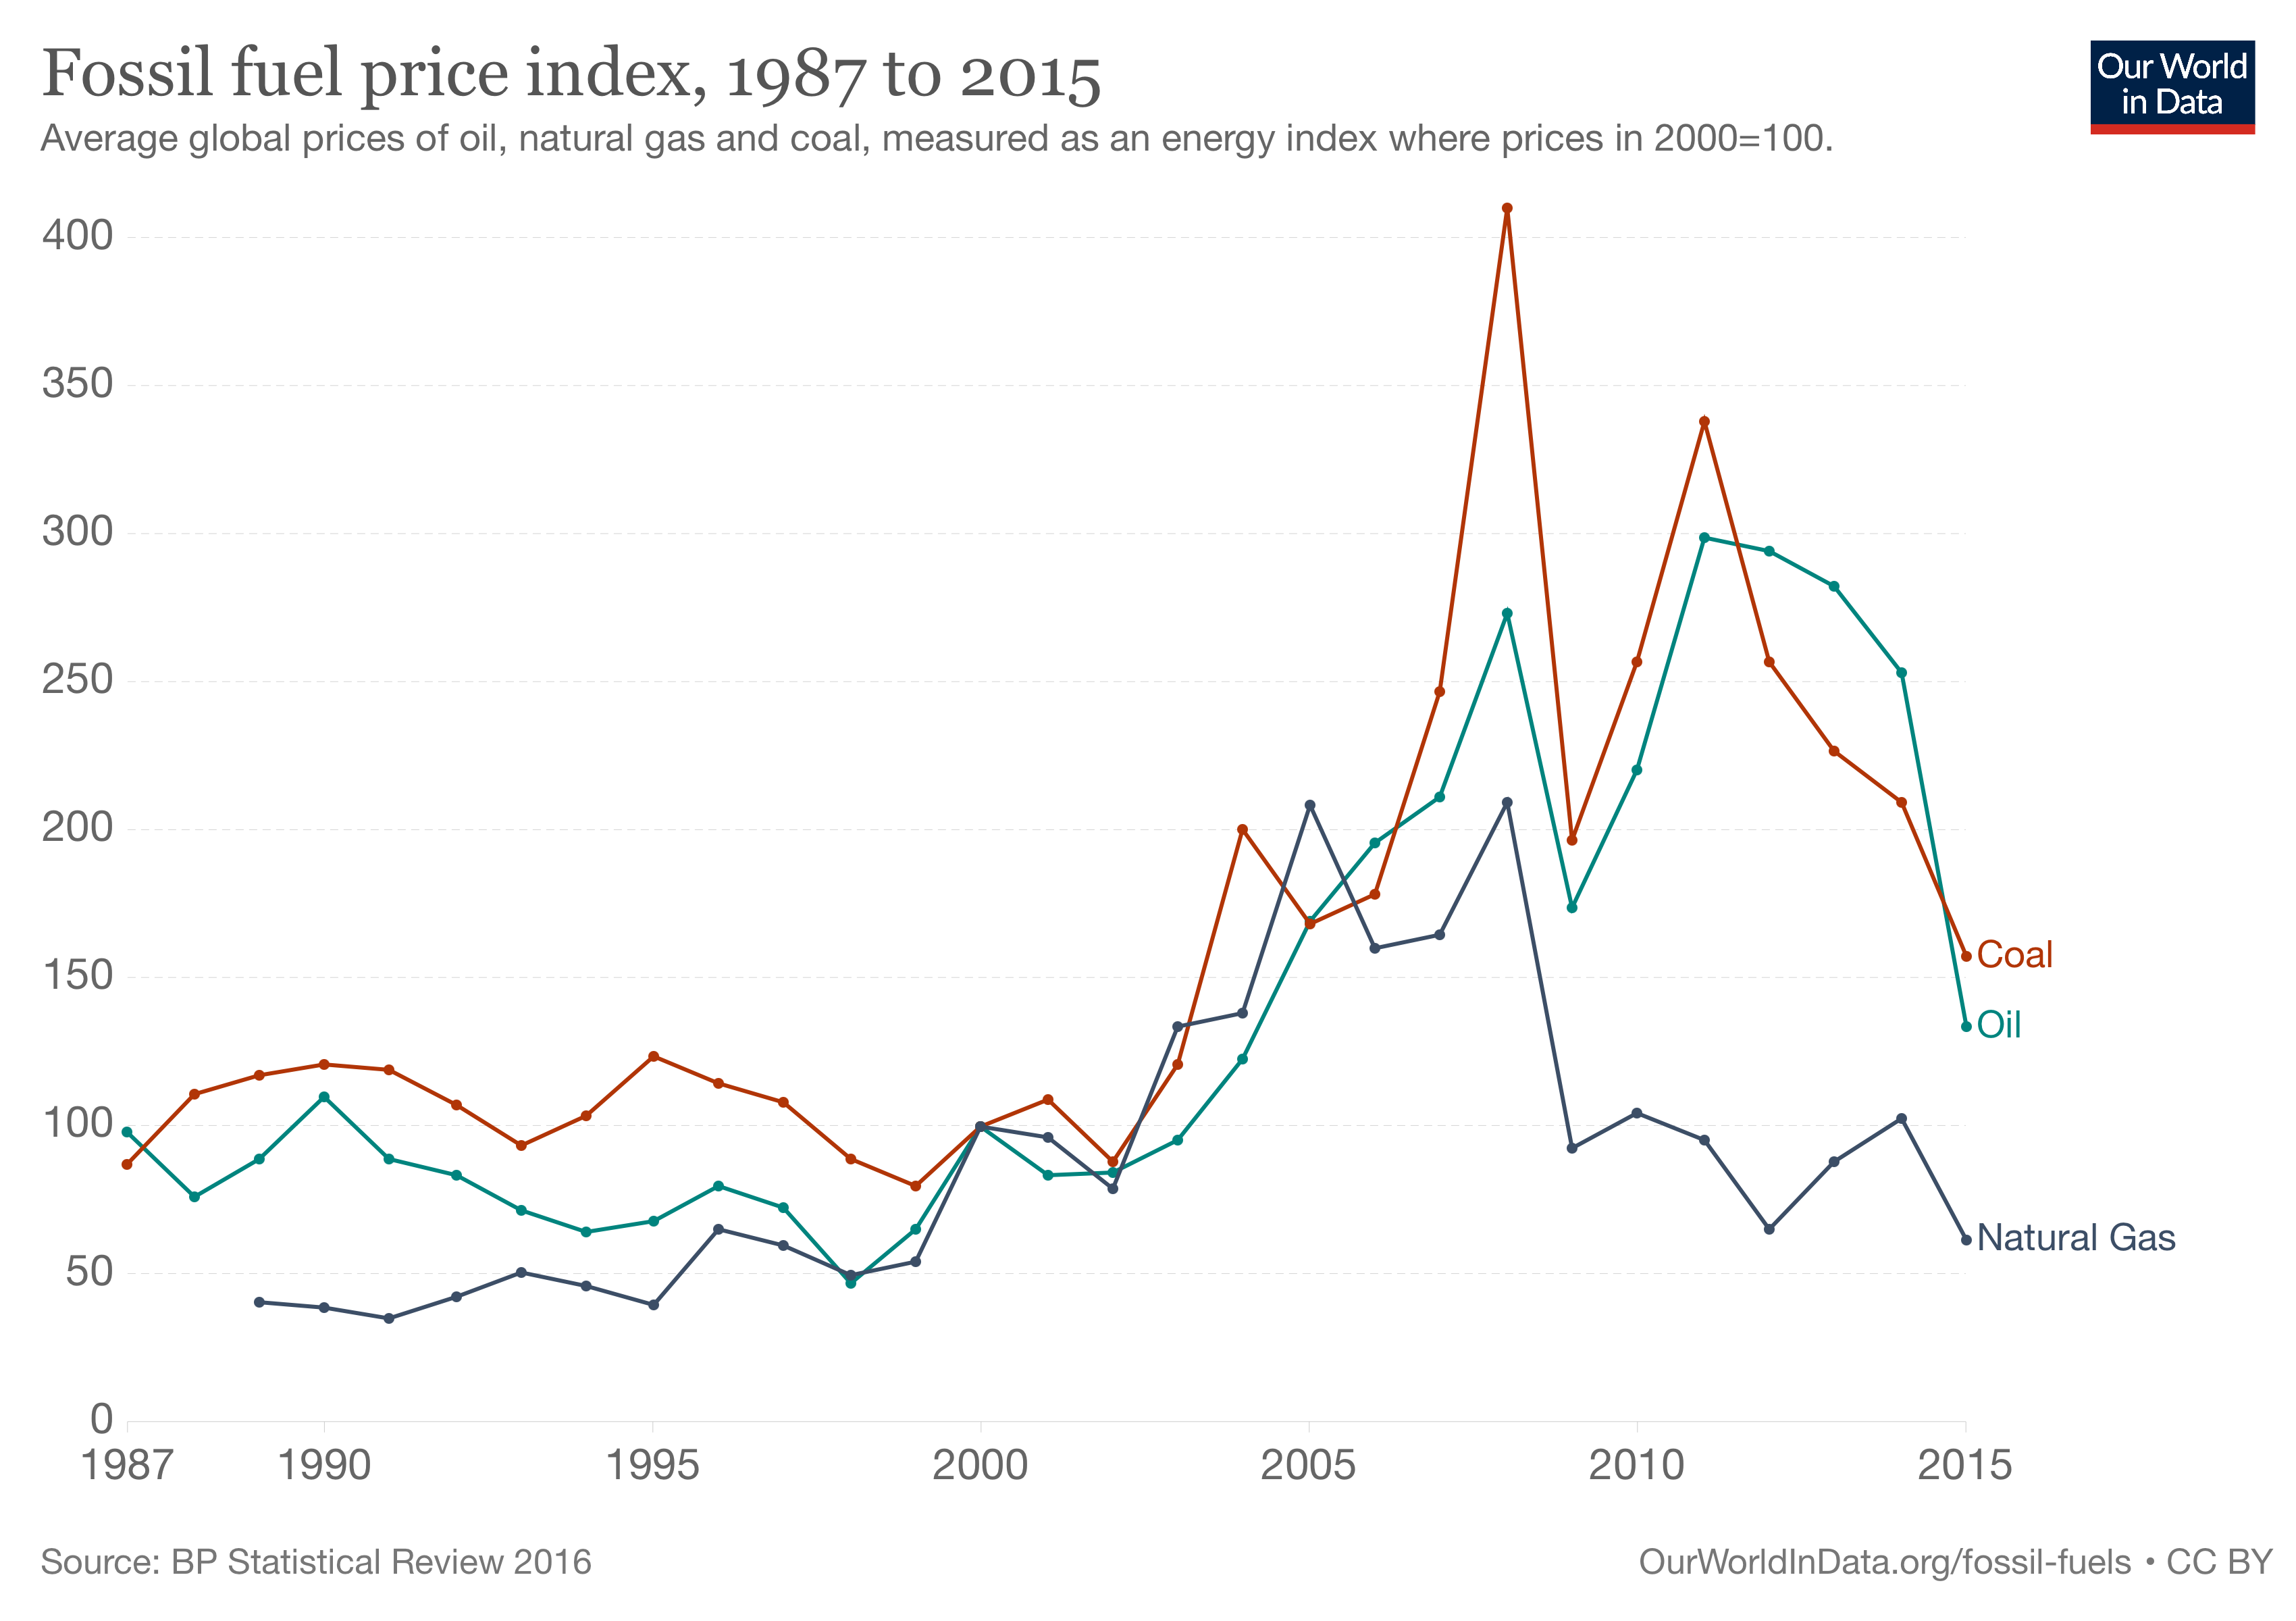
\includegraphics[scale=0.11]{img/intro_fossil-fuel-price-index.png}
\caption{Prices of different fossil fuels rose from 1987 to 2015 overall~\cite{BP2016bp}.}
\label{intro_fossil-fuel-price-index}
\end{figure} % Figure 1.2

Although we might not meet the complete depletion of non-renewable resources in the future 50 years, based on Hotelling’s "Economics of Exhaustible Resources", David Ricardo proposed that as the historical production stock accumulates, higher grade ores get depleted, and the producer resorts to lower grade ores, sustaining greater extraction costs~\cite{devarajan1981hotelling}. It means the extraction costs rise, and the price of the products based on ores will rise as well. Thus, we can assume that the price of most non-renewable resources, like oil, coal and gas, will rise since these have similar properties with ores. In fact, according to BP Statistical Review 2016, from 1987 to 2015 (from 1989 to 2015 for natural gas), the price of oil, coal and natural gas rose by approximately 36\%, 81\%, and 53\% overall (Figure~\ref{intro_fossil-fuel-price-index}). \\

The climate on the earth has changed throughout history. Just in the past 650,000 years, there were seven-cycle glaciers to advance and retreat. As shown in Figure~\ref{intro_co2-concentration-long-term}, however, atmospheric \ce{CO2} had never been above 300 parts per million until the year 1950. According to the paper from Nature, the climate has been changed differently from other periods that happened in the past 70 years~\cite{parmesan2003globally}. It has already had effects on the environment around us. Glaciers are shrinking, and ices are breaking up earlier on the lakes and rivers. Most climate scientists agree that it is human activities that cause global warming~\cite{epic337530}. The atmospheric concentration of \ce{CO2} has been risen for around 36\% since 1914 (see Figure~\ref{intro_co2-concentration-long-term}). As we know, \ce{CO2} is a significant component of the atmosphere. More than a third has increased atmospheric \ce{CO2} concentration since the Industrial Revolution began~\cite{epic337530}. More importantly, as shown in Figure \ref{intro_nasa_co2}, atmospheric \ce{CO2} has exceeded the highest level in the past 400,000 years, and it was 408.52 ppm in 2018. \\

\begin{figure}
\center
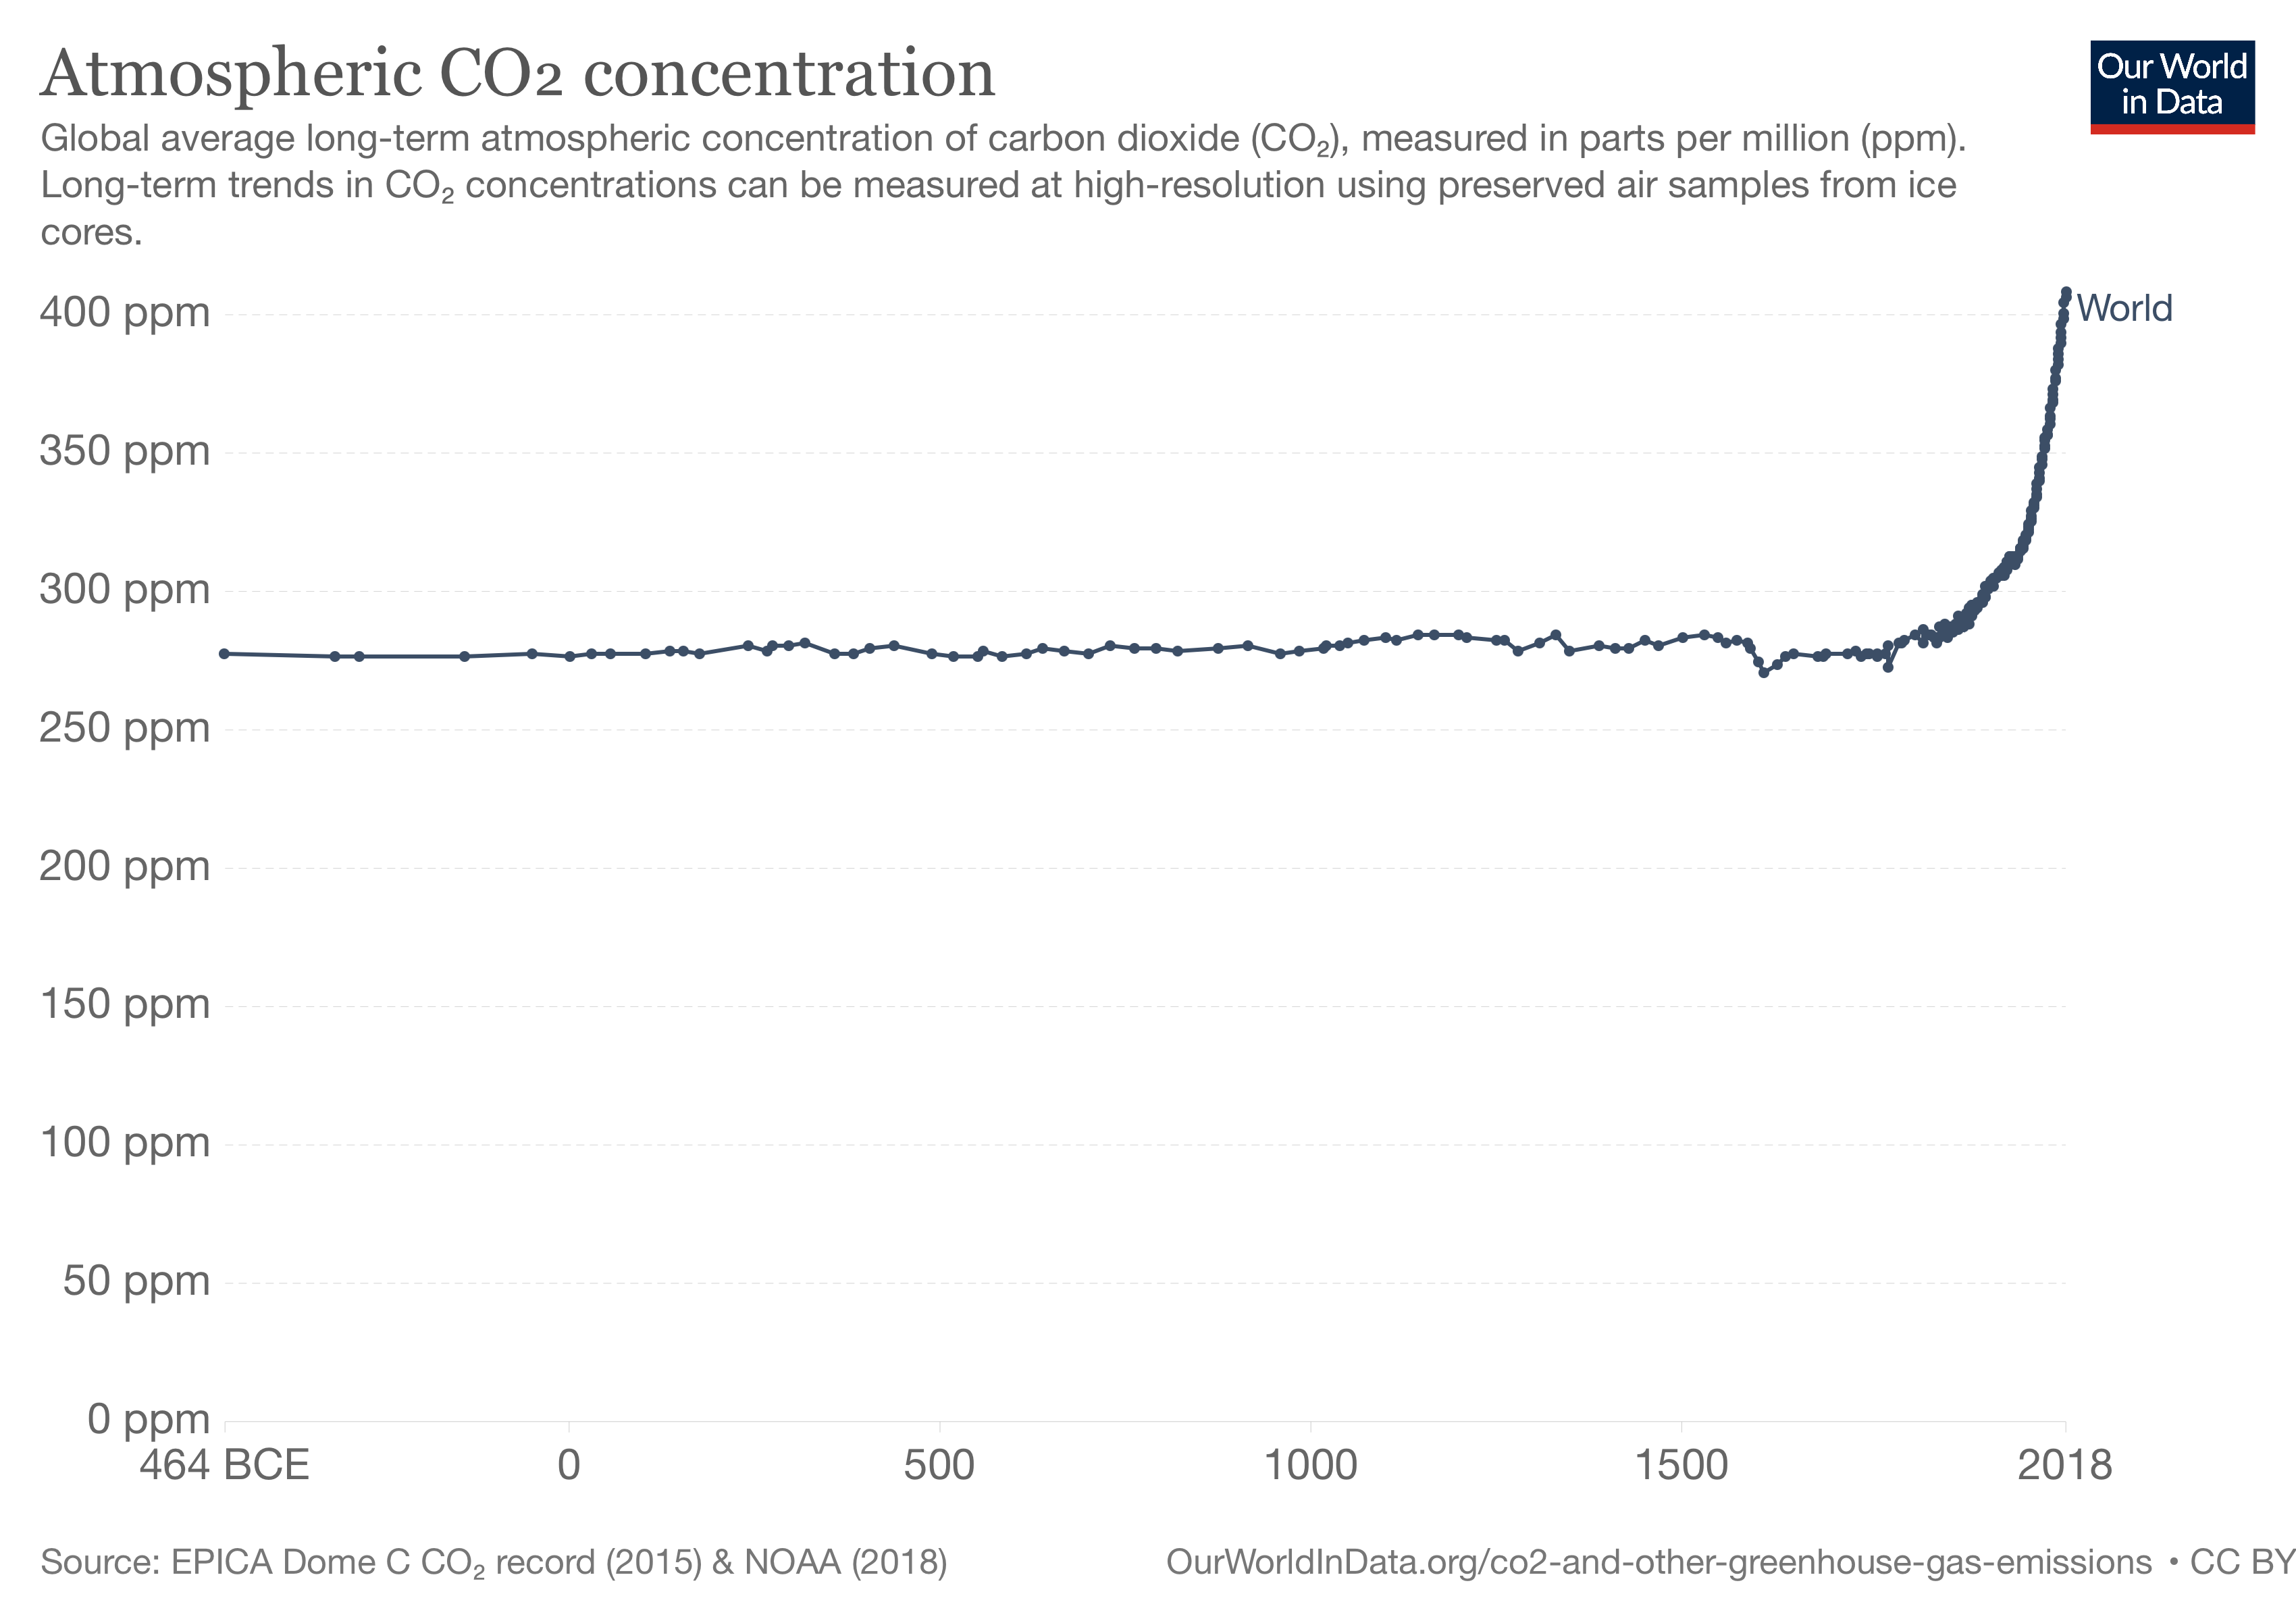
\includegraphics[scale=0.12]{img/intro_co2-concentration-long-term.png}
\caption{Atmospheric concentration of \ce{CO2} since 564 BCE~\cite{bereiter2015revision}. Atmospheric concentration of \ce{CO2} in 1914: 300.17ppm; Atmospheric concentration of \ce{CO2} in 2018: 408.52ppm.}
\label{intro_co2-concentration-long-term}

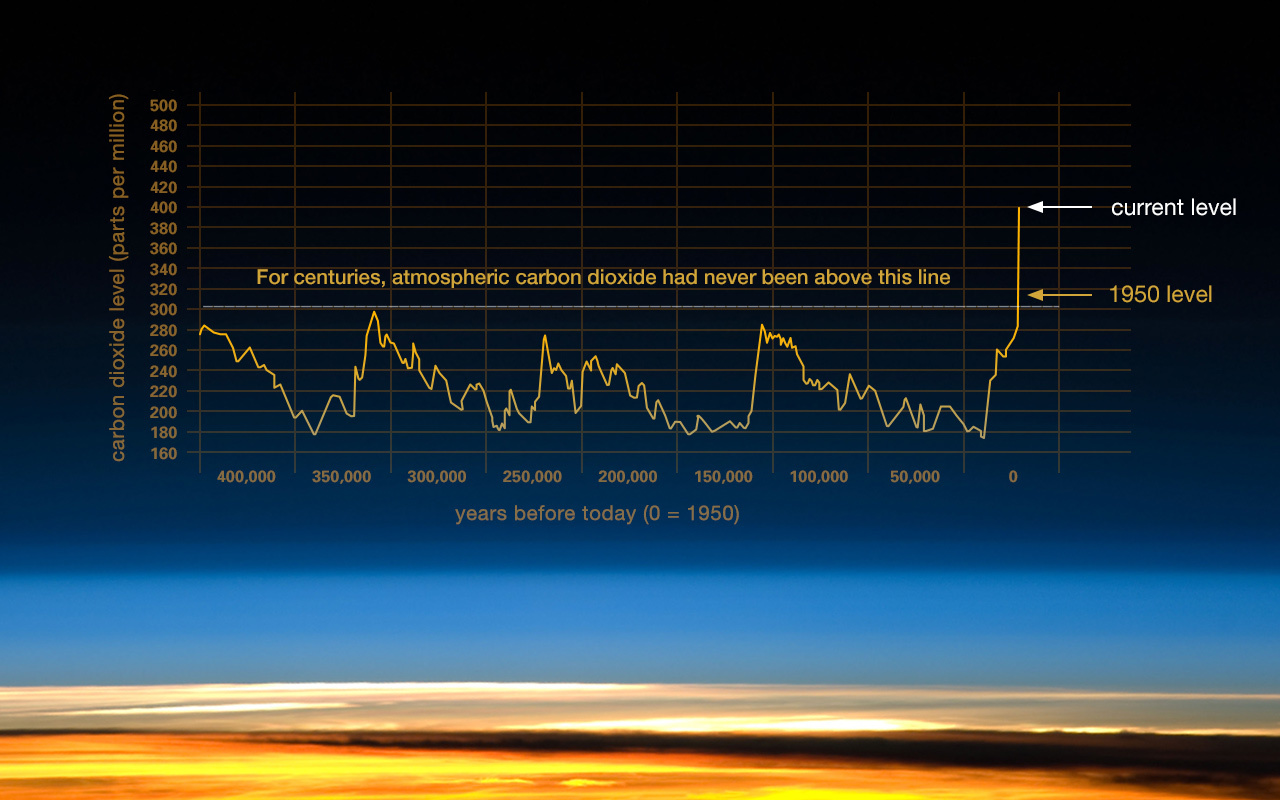
\includegraphics[scale=0.33]{img/intro_nasa_co2.jpeg}
\longcaption{The evidence that atmospheric \ce{CO2} has increased since the Industrial Revolution began}{\label{intro_nasa_co2} The evidence that atmospheric \ce{CO2} has increased since the Industrial Revolution began. Image courtesy: https://climate.nasa.gov/evidence}
\end{figure}


In summary, the rising energy demand and lack of energy supply may cause a short-term energy crisis. The finite resources of fossil energy will drive the price of electricity and consumer goods to rise. The burning of fossil energy will cause excessive emissions of greenhouse gases, leading to global warming. However, a door opens for cheaper but unpredictable renewable energy due to a more expensive fossil fuel. According to Paris Agreements~\cite{unies2015accord}, it is vital to reduce the emissions of fossil energy on a large scale in every sector of human activities. To respond to climate change, supporting the United Nations Sustainable Development Goals and taking urgent action to address climate change and its impact, the International Maritime Organization has formulated a timetable to reduce greenhouse gas emissions from international shipping.~\cite{joung2020imo} It pointed out that between 2030 and 2050, the carbon intensity of the fleet will be reduced by at least 70\%~\cite{joung2020imo}. Before 2050, the total annual greenhouse gas emissions will be reduced by at least 50\%, which requires a reduction of approximately 85\% of carbon dioxide per ship~\cite{joung2020imo}.\\ 

\newpage
\subsection{Small-Boat Fleet and Emission Inventory}
In 2018, total shipping \ce{CO2} emissions increased to 1056 million tonnes compared to 962 million tonnes in 2012~\cite{IMO2021Fourth}.
In 2016, total \ce{CO2} emissions of the industrial fishing sector were 159 million tonnes, and the small-scale fishing sector emitted 48 million tonnes~\cite{GREER2019103382}. Suppose the increase rate of \ce{CO2} in 2018 was the same as the rate in 2016, and the ratio of the number of small boats and the number of boats can be approximate as the ratio of the number of small fishing boats and the number of fishing boats. Then in 2018, the total \ce{CO2} emissions for the small boat fleet can be calculated as 318.8 million tonnes.\\

Small vessels are classified as those smaller than 24 meters~\cite{uk2021Operational}. Knowing the emissions inventory of the shipping sector can help to understand what measures need to be taken to enable the industry to start the road to full decarbonization. Although it is possible to calculate large vessels from the international registry system and use the satellite data sent from the ship's transponder to account for the numbers of the large vessels~\cite{IMO2021Fourth}, the small vessels depend on the national registration system, and their operation is assumed. In addition, there are many types of small vessels fleets such as machinery (e.g. fishery, people carrier, etc.), hull shape and structure, and the activities of owners and operators. The diverse small boat fleet operational profile is increasing the challenge of accurately accounting for their emission inventories.\\

Emissions from the global fishing industry grew by 28\% between 1990 and 2011, with a minor coinciding increase in production; however, marine fisheries are typically excluded from international assessments of \ce{CO2} or are generalized based on a limited number of case studies~\cite{parker2018fuel}. Developed economies such as the UK have a national registry~\cite{uk2021registration} that allows to have a sense of the level of small boat activity and hence infer the \ce{CO2} emissions.\\

However, in developing countries, it tends to be a mixed bag on the level of precision and availability. For instance, in Mexico, only fishing vessels are counted into registry~\cite{Mexico2021RegisteredVessels}. Still, it is difficult to know where they are located. Besides, the rest of the small-boat fleets are not considered. In all, Mexico does not have a regional \ce{CO2} inventory considering the small-boat fleet. Therefore, quantifying the number of small-boat fleets will allow a better precision of where the emissions are being emitted and will be the focus of understanding the emission inventory of the shipping sector.\\


Observing the shipping activity in the Gulf of California is essential due to its unique geographical location, conformation, and biophysical environment ~\cite{LLUCHCOTA20071, munguia2018ecological, MARINONE2012133}. In the Gulf of California, there is the largest fish producing state (Sonora) in Mexico~\cite{MELTZER2006222} and the most prominent sports fishing destination (Los Cabos, Baja) in Mexico~\cite{hernandez2012economic}. Besides, the Gulf of California has a faster shipping route to mainland Mexico than from Yucatán Peninsula.\\




%\section{Thesis Outline}


%\section{Contributions}

% Literature Review
\chapter{Literature Review}
\label{chapter:review}
%!TEX root = thesis.tex

\section{Small Boat Fleet and Shipping Decarbonisation}
Current literature related to estimating small-scale vessels without machine learning methods includes using statistical factor or measure.~\newcite{johnson2017spatial} used Kernel Density Estimation (KDE) to distribute data on the population, the number of ships, and the average annual total catch for the entire population, and finally showed that their forecasts could accurately predict the landing of fisheries in the bay. However, another point to make against this work is that it only focuses on fishing vessels. While these are the majority, it still misses the other ship types. Notably, the authors provided information (Figure~\ref{review_density_of_gulf}) of the density of human population and boats in the Gulf of California that can save much time in creating data sets of the Gulf of California for training machines learning models.\\

\begin{figure}[t]
\center
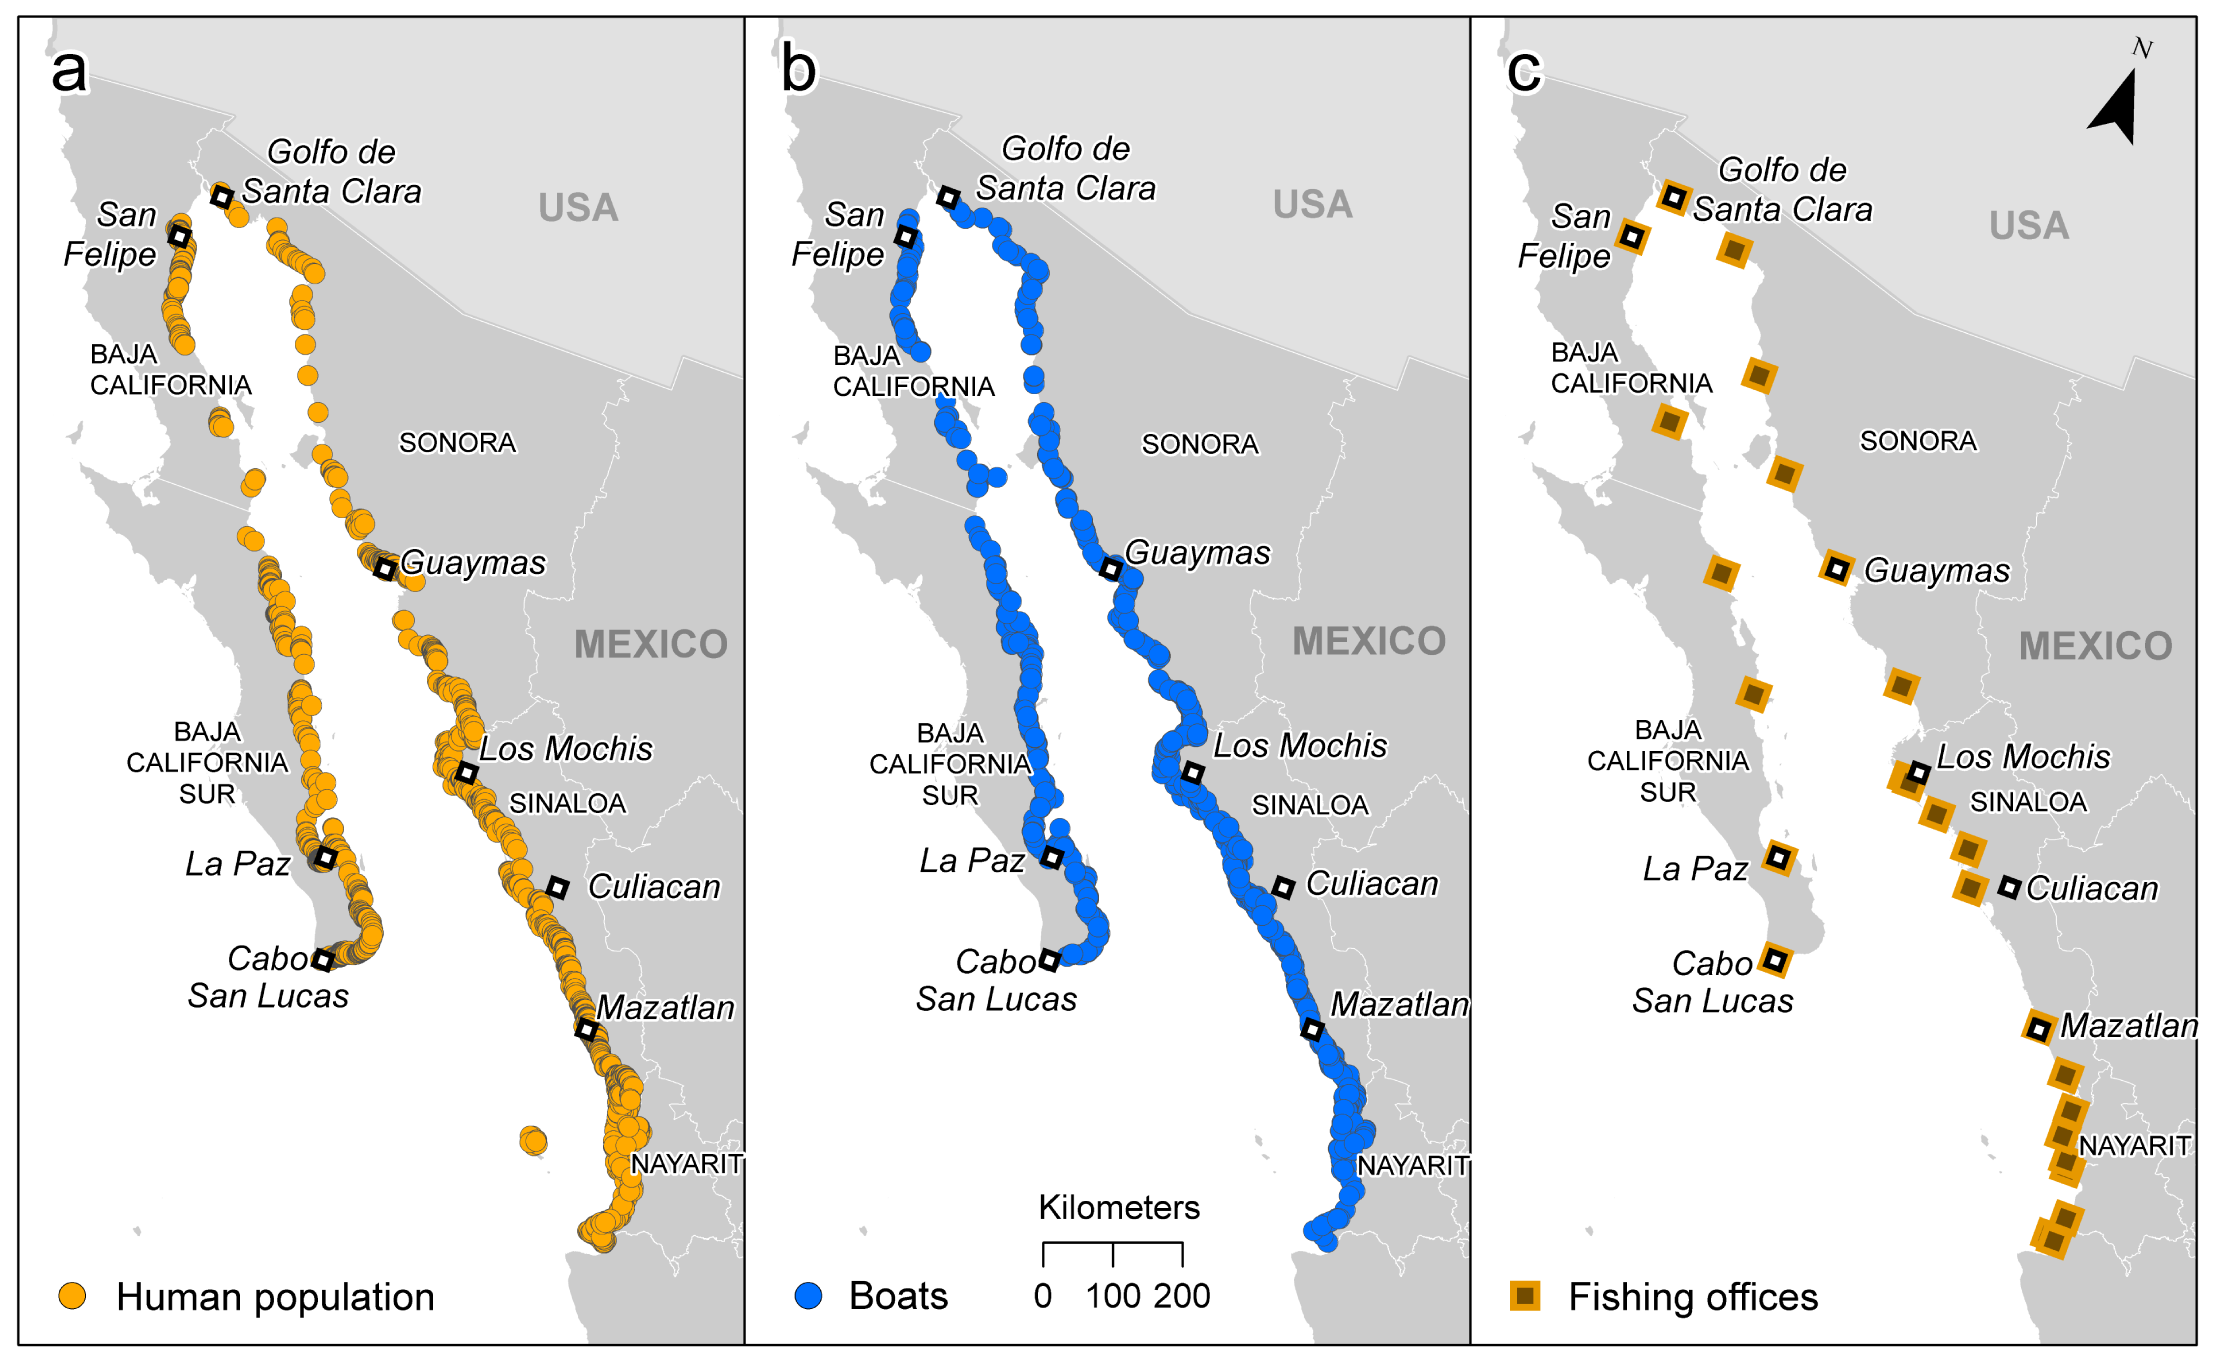
\includegraphics[scale=0.83]{img/review_density_of_gulf.png}
\longcaption{Map of the density of human population, boats, and fishing offices in the Gulf of California.}{\label{review_density_of_gulf} Map of the density of human population, boats, and fishing offices in the Gulf of California. Image courtesy: https://doi.org/10.1371/journal.pone.0174064.g002}
\end{figure}

~\newcite{Johansson2018ModelingOL} proposed a new model (FMI-BEAM) to describe the emissions of the leisure boat fleet in the Baltic Sea region with over 3000 dock locations, national small boat registry, AIS data and vessel survey results. However, the method cannot cover countries with no national registry for small boats. Besides, small boats are not just leisure boats.~\newcite{Ug2020EstimationOW} estimated global ship emissions with the help of data from the Automatic Identification System (AIS). They set up movement information relating to ship size and speed and meteorological and marine environmental conditions. Over 3,000,000,000 daily AIS data records from hundreds of owners and thousands of partner AIS base stations and detailed ship data. However, this method is highly dependent on AIS data which is impossible for unregistered small boats.~\newcite{Traut2013MonitoringSE, Johansson2016ACM, Mabunda2014EstimatingCD, Hensel2020GreenSU, Han2016RealtimeIA} have proposed the use of AIS to monitor the carbon emissions of the fleet as well.\\

~\newcite{Zhang2019TheSO} included unidentified vessels in the AIS-based vessel emission inventory. They developed an AIS-instrumented emissions inventory, including both identified and unidentified vessels. In particular, missing vessel parameters for unidentified vessels were estimated from a classification regression of vessels with similar vessel types and sizes in the AIS database. However, the authors do not discuss whether the regression model applies to vessels in most coastal areas of the planet. In addition, the authors do not discuss whether the vessel data in the AIS database is regionally diverse. Finally, if there is a diversity of vessels in the AIS database, the authors did not discuss whether this diversity would produce more significant errors in the predictions for small vessels in a single region (e.g. the Gulf of California, Mexico).


\section{Convolutional Neural Networks in Image Recognition}
Literature tends to be inaccurate for emission inventories for the small boat fleet. I am covering the closest to detecting the activity level, but I want to go one step further into emissions. The use of available satellite imagery and advanced image recognition algorithms will allow researchers to identify small boats in any sea area, significantly reducing the time taken to calculate small vessel emission inventories. Besides, it will be in the national interest for the small fleet to account for and control these emissions within the powers of the state, incentivising the uptake of technology. Further, if countries are to meet their ambitious net-zero carbon emissions targets, they cannot afford to ignore image recognition algorithms that can help governments account for carbon emissions from small boats more quickly.\\

Object detection is an active topic in image recognition and computer vision. In the past few years, this topic has made significant progress. With the rise of self-driving cars and face detection, there is an increasing demand for fast and accurate objects detection. In 2012, AlexNet won the ImageNet Large-Scale Visual Recognition Challenge (ILSVRC), making convolutional neural networks the dominant mode of image recognition~\cite{krizhevsky2012imagenet}. Then,~\newcite{girshick2014rich} introduced R-CNN, which is the first CNN-based object detection method, but with higher performance.\\

Unlike other deep learning problems, the unknown number, size and categories of instances in each image in the object detection problem lead to unexplored dimensions of the model output. Therefore, it is not easy to adapt the classic deep learning classification model that expects a fixed output size to the object detection problem. Region-Based Convolutional Neural Networks (R-CNN) may be the way to meet this challenge.\\

Since its inception, Region-Based Convolutional Neural Networks (R-CNN) has gone through many iterations: R-CNN, Fast R-CNN, Faster R-CNN and Mask R-CNN~\cite{girshick2014rich, girshick2015fast, ren2015faster, he2017mask}. To avoid computationally expensive, pixel-level classification and object search, the original R-CNN method applied a non-deep learning algorithm called Selective Search to obtain approximately 2000 region suggestions~\cite{uijlings2013selective, girshick2014rich}. Then, with the help of a modified version of the AlexNet model, features are extracted from the proposed region. The objects in the image have different scales and sizes, so their corresponding image crops need to be warped to fit the following CNN input size. Then, the support vector machine (SVM) classifier uses the extracted features for classification, and the linear regression predicts the offset of the bounding box, thereby tightening the bounding box around the object~\cite{girshick2014rich}.\\

R-CNN is an intuitive architecture that has achieved high accuracy in object detection. However, since the reasoning time for each image is about 30 seconds, this model is very inefficient for applications that require real-time prediction~\cite{huang2017speed}. Fast R-CNN performs feature extraction on the image before generating the region suggestion. The region suggestion is generated based on the final feature map instead of the original image itself, significantly improving the training and inference speed. Therefore, only one CNN forward channel is calculated on the entire image, instead of about 2000 channels as it is now. Although Fast R-CNN does improve efficiency, selective search to generate region recommendations is the most computationally intensive part of the architecture, which forms a bottleneck in network inference and training time. Faster R-CNN alleviates this problem by replacing the selective search algorithm with a neural network called a region proposal network (RPN). The network simultaneously predicts the boundaries of objects and the classification between the two types of objects at each location and the background~\cite{ren2015faster}. The rest of the architecture is similar to that proposed by Fast R-CNN.
A recently proposed architecture, Mask R-CNN~\cite{he2017mask}, can perform object detection in addition to instance segmentation by adding a fully convolutional network (FCN) branch to the Faster R-CNN architecture. Instance segmentation can be defined as demarcating and classifying object instances belonging to different categories in the image.\\

However, even traditional CNNs can be very useful for large-scale image recognition.~\newcite{Simonyan2015VeryDC} in the University of Oxford, and Google DeepMind researched the effect of convolutional network depth on its accuracy in the large-scale image recognition setting. Their research found out that even they used very small (3x3) convolution filters, a significant improvement can be achieved by pushing the depth to 16 to 19 weight layers.\\


\section{Noise Removal for Image in the Shipping Sectors or Similar Applications}
Satellite images often have targets that should not be there, such as shadows cast by water on the sea surface due to sunlight or clouds in the atmosphere. These noises can make the training data inaccurate and often cause problems for the correctness of the model.~\newcite{He2009SingleIH} proposed a simple but effective image prior-dark channel before removing haze from a single input image. The dark channel prior is a kind of statistics of outdoor haze-free images. It is based on critical observation-most local patches in outdoor haze-free images contain some pixels whose intensity is very low in at least one colour channel. Using this prior to the haze imaging model, the thickness of the haze can be estimated, and a high-quality haze-free image can be recovered. Moreover, a high-quality depth map can also be obtained as a byproduct of haze removal.\\


%\section{Image Segmentation in the Shipping Sectors or Similar Applications}






% Conclusion
%\chapter{Conclusions}
%\label{chapter:conclusions}
%%!TEX root = thesis.tex



% Bibliography
\bibliographystyle{bartlett_harvard_ref}
\bibliography{ref}

\end{document}
